\documentclass[a4paper,12pt]{article}
\usepackage{polski}
\usepackage[utf8]{inputenc}
\usepackage[left = 3cm, right = 3cm, top = 2cm, bottom = 2cm]{geometry}
\usepackage{enumerate}
\usepackage{amssymb}		% pakiet do symboli
\usepackage{mathtools}		% pakiet do matmy (rozszerza amsmath)
\usepackage{enumitem}		% punktowanie (a), (b), ...
\usepackage{nopageno}		% brak numerow stron
\usepackage{graphicx}		% wstawianie obrazkow
\usepackage{float}			% wstawianie obrazkow w dowolnym miejscu
\usepackage{caption}
\usepackage{esdiff}         % pochodne \diff{}{}
\usepackage{listings}
\usepackage{xcolor}
\usepackage{adjustbox}
\usepackage{tkz-graph}
%\usepackage[none]{hyphenat} % usunięcie łamania wyrazów na końcu linii

% nowe komendy dla wygodniejszego pisania :)

\newcommand{\floor}[1]{\left\lfloor #1 \right\rfloor}	% podłoga
\newcommand{\ceil}[1]{\left\lceil #1 \right\rceil}		% sufit
\newcommand{\fractional}[1]{\left\{ #1 \right\}}		% część ułamkowa {x}
\newcommand{\abs}[1]{\left| #1 \right|}					% wartosc bezwzgledna / moc
\newcommand{\set}[1]{\left \{ #1 \right \}}				% zbiór elementów {a,b,c}
\newcommand{\pair}[1]{\left( #1 \right)}				% para elementów (a,b)
\newcommand{\Mod}[1]{\ \mathrm{mod\ #1}}				% lekko zmodyfikowane modulo
\newcommand{\comp}[1]{\overline{ #1 }} 					% dopełnienie zbioru 
\newcommand{\annihilator}{\mathbf{E}}					% operator E
\newcommand{\seqAnnihilator}[1]{\annihilator \left\langle #1 \right\rangle} % E(a_n)
\newcommand{\sequence}[1]{\left\langle #1 \right\rangle} % <a_n>
\DeclareMathOperator{\lcm}{lcm}							% obsługa lcm w mathmode

% styl do kodu
\lstdefinestyle{code}{%
basicstyle=\ttfamily\small,
commentstyle=\color{green!60!black},
keywordstyle=\color{magenta},
stringstyle=\color{blue!50!red},
showstringspaces=false,
numbers=left,
numberstyle=\footnotesize\color{gray},
numbersep=10pt,
tabsize=4,
rulecolor=\color{red},
breaklines=true
}

\newcommand{\code}[1]{\lstinline[style=code]{#1}} % kod inline

\begin{document}
\noindent \textbf{Matematyka dyskretna L, Lista 11 - Tomasz Woszczyński}\newline

\noindent \newline \textbf{Zadanie 8} \newline
Mamy $2n$ uczniów, z których każdy ma przynajmniej $n$ przyjaciół. Pokaż, że można ich
usadzić w $n$ ławkach tak, by każdy z nich siedział z przyjacielem. Pokaż też, że jeśli
$n > 1$, to może być to zrobione na co najmniej dwa sposoby. \\

\noindent Twierdzenie Diraca: jeśli graf jest prosty i $n \geq 3$ oraz jeśli dla każdego
wierzchołka $v$ zachodzi $\deg(v) \geq \frac{n}{2}$, to jest on hamiltonowski (a więc
zawiera cykl przechodzący przez każdy wierzchołek dokładnie raz). \\

\noindent Korzystając z tego twierdzenia wiemy, że w tym grafie musi być cykl Hamiltona.
W tym cyklu krawędzie oznaczają możliwe usadzenia przyjaciół w ławkach. Aby wybrać kto
z kim siedzi, musimy wziąć co drugą krawędź (jako że jedna osoba nie może siedzieć
w dwóch miejscach jednocześnie). Możliwości na wybranie co drugiej krawędzi mamy dwie,
co kończy dowód.

\noindent \newline \textbf{Zadanie 10} \newline
Pokaż przykład grafu pokazujący, że założenie $\deg(v) \geq \frac{n}{2}$ w twierdzeniu
Diraca nie może być zastąpione słabszym założeniem $\deg(v) \geq \frac{n-1}{2}$. \\

\noindent Weźmy graf przedstawiony poniżej. Ma on $5$ wierzchołków, czyli $n = 5$, a 
wartości stopni wszystkich wierzchołków są następujące: $\{ 2, 2, 2, 3, 3 \}$. Oznacza 
to, że wszystkie wierzchołki spełniają słabszy warunek, a więc $\deg(v) \geq 
\frac{n-1}{2}$. W naszym grafie jednak nie da się znaleźć cyklu Hamiltona, co możemy 
udowodnić usuwając wierzchołki $\{ 2, 3 \}$ - graf zostanie podzielony na $3$ spójne 
składowe, więc ścieżka Hamiltona nie może w nim istnieć.

\begin{figure}[h]
    \centering
    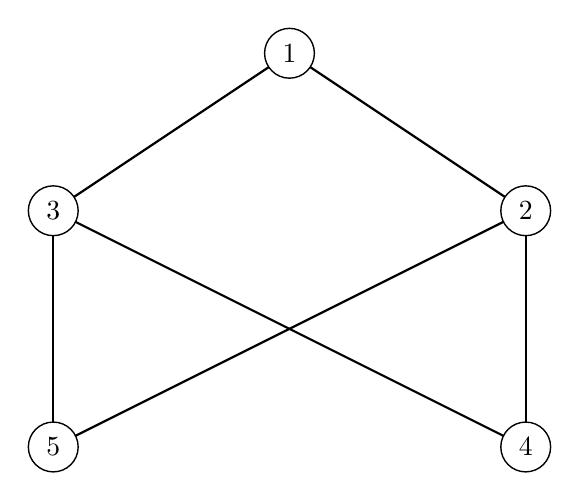
\begin{tikzpicture}
        \Vertex[x=0, y=0]{1}
        \Vertex[x=3, y=-2]{2}
        \Vertex[x=-3, y=-2]{3}
        \Vertex[x=3, y=-5]{4}
        \Vertex[x=-3, y=-5]{5}
        \Edge[](1)(2)
        \Edge[](1)(3)
        \Edge[](2)(4)
        \Edge[](2)(5)
        \Edge[](3)(4)
        \Edge[](3)(5)
    \end{tikzpicture}
\end{figure}


\end{document}